\subsection{Primal Dual Algorithm}

Next we'll look at a primal dual algorithm for the Set Cover problem. We assume that no element is contained in more than $f$ sets. We'll construct a solution to the ILP and a feasible solution for the dual and relate their costs.

The algorithm is as follows:

\begin{lstlisting}
for all $e$
	$y_e=0$ //dual variables
while $\exists$ uncovered element
	$e$ = uncovered element
	raise $y_e$ until a packing constraint becomes tight
	add all tight sets to the cover
	set added elements to covered
\end{lstlisting}

The algorithm is very easy to analyse. Because we only add tight sets we have

\begin{align*}
\sum_{S \text{ in cover}} c_s  &= \sum_{S \text{ in Cover}} \sum_{e\in S} y_e\\
	&=\sum_{e} y_e \cdot \text{\# of sets in cover containing e}\\
	&\leq \sum_{e} y_e \cdot f\\
	&= f\cdot OPT
\end{align*}

So this algorithm is a $f$ approximation.

\section{Steiner Tree Problem}

This is a bit similar to the Minimum Spanning Tree. We want to connect a set of $T$ terminals as cheaply as possible, but we are allowed to use edges from a larger graph $G$ in which $T$ are embedded.

\subsection{Auxiliary Graphs}

We can use the following approach

\begin{enumerate}
\item Construct a complete graph on $T$. The edges have weight $d(u,v)$ equal to the weight of the shortest path in $G$ between $u,v$.
\item Construct a MST in the auxiliary graph
\item Interpret the MST in G, i.e. replace edges by shortest paths.
\end{enumerate}

Because the shortest paths needn't be edge disjoint the weight of the MST in the auxiliary graph is larger than the optimal solution in $G$.

We want to show that it is at most twice the cost of the Steiner Tree. The argument works similar to the argument for the approximation guarantee of the Christofides approximation.

\begin{figure}[hbt]
\begin{center}
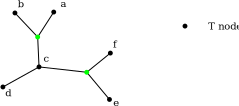
\includegraphics{./images/steinerTree}
\end{center}
\caption{A optimal solution for the Steiner Tree problem}
\label{fig:steinerTree}
\end{figure}

Have a look at figure \ref{fig:steinerTree} and consider the following path in the auxiliary graph

\[(a,b),(b,c),(c,d),(d,e),(e,f)\]

Because we take shortest paths the auxiliary graph we get the desired approximation.

\subsection{Steiner Forests}

Instead of wanting connections between all nodes in some set $T$ we have a $k$ pairs $(s_i,t_i)$ which we want to connect as cheaply as possible, i.e. select edges such that there is a path from $s_i$ to $t_i$ for all $i$.

We introduce some notation: For $S\subset V$

\[\delta(S) = \{(u,v)\in E |\ |S\cap \{u,v\}| = 1\}\]

is the is boundary of $S$, i.e. all edges that have exactly one endpoint in $S$. Further let 

\[f(S) = \begin{cases}
1 & \exists i |S \cap \{s_i,t_i\}| =1\\
0 & \text{otherwise}
\end{cases}\]

$f(S)$ is zero if S is \emph{saturated}. If $S$ is not saturated we need to pick one edge from the boundary.

The ILP for the Steiner Forest problem looks like this: We introduce decision variables $x_e$ for all edges

\begin{align*}
\min \quad & \min c_e x_e\\
s.t. \quad & \sum_{e\delta(S)} x_e \geq 1  && \forall S, f(S)=1\\
	& x\in \{0,1\}
\end{align*}

It is clear that any solution for the problem satisfies the constraints. If we have a solution for this ILP this must also be a solution to the problem. Assume there is a $s_i$ that is not connected to $t_i$. Then let $S$ be the reachable set from $s_i$. This must be unsaturated and no edge from the boundary is picked, hence the constraint for this $S$ must be violated.

We know consider the LP relaxation to form the dual. In the dual we get a variable $y_s$ for each unsaturated $S$.

\begin{align*}
\max \quad & y_s\\
s.t.\quad & \sum_{S;e\in \delta(S)} {y_s} \leq c_e\\
\end{align*}

Note that this LP has an exponential number of variables. As we'll see shortly this does no harm, as we don't look at most of them at all.

We now again construct a primal-dual algorithm that constructs a feasible solution to the dual and a set of $F$ of edges. $F$ will be a forest.

We will then extract a primal solution from $F$ by pruning edges.

At any step of the algorithm we have a collection of sets called \emph{current sets}. They partition $V$. A current set is active if it is unsaturated, passive if it is saturated. We initialise the collection with the singleton sets. Active are all those that contain $s_i$ or $t_i$. 

While there is an active constraint we increase the dual variables of all active sets until one edge becomes tight. $F$ will denote the set of edges already picked, intially it is empty.

The current sets are the connected components of $(V,F)$. For all $e=(u,v)$ such that $u$ and $v$ belong to distinct components $C_u,C_v$ of $(V,F)$. Define

\[\epsilon(e) = \frac{c_e - \sum_{e\in \delta(S)} y_S}{f(C_u)+f(C_v)}\]

to be the maximum amount we can increase dual variables until the edge $(u,v)$ between the two components becomes tight. Let 

\[\epsilon = \min \{\epsilon(e)|e=(u,v) \text{connects different components}\}\]

Let $e$ be the edge that minimises $\epsilon(e)$. We add $e$ to $F$, make $C_u,C_v$ inactive, remove them from the active sets and add $C_u\cup C_v$ to the current sets.

\begin{lstlisting}
Current Sets = $\{v\},\ v\in V$
while $\exists$ active set
	$F = e \cup F$ $e$ minimises $\epsilon(e)$
	for every active set $S$
		$y_s = y_s + \epsilon$
	$C_u$, $C_v$ become inactive and are no longer current
	$C_u \cup C_v$ becomes current set

$F'=\{e\in F| \text{in }F\backslash e\text{ some pair } (s_i,t_i)\text{ is not connected}\}$
\end{lstlisting}

\begin{Ex} We run the algorithm on an example instance
The sequence of steps looks like in figure \ref{fig:steinerTreePrimalDual}

\begin{figure}[hbt]
\begin{center}
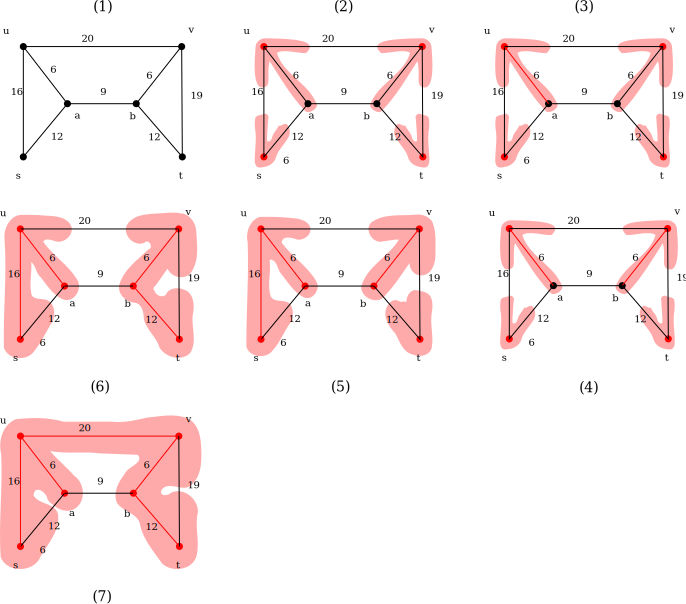
\includegraphics[width=\linewidth]{./images/steinerPrimalDual}
\end{center}
\caption{A run of the Primal-Dual Algorithm}
\label{fig:steinerTreePrimalDual}
\end{figure}

The algorithm works as follows:

\begin{enumerate}
\item The initial graph. We want to connect $(u,v),(s,t)$. Hence the singletons containing them are active.
\item We increase $y_u,y_v,y_s,y_t$ to 6 because then the edges to $a$, $b$ become tight.
\item Arbitrarily pick edge $(u,a)$. $\{u,a\}$ becomes active, $\{u\}$ becomes inactive. Increase everything by $0$, because there is already a tight edge.
\item Pick $(v,b)$, $\{v,b\}$ becomes active $\{v\}$ inactive.
\item Increase everything by 2 because the edge $(u,s)$ becomes tight, as 
\[16 - y_{u} - y_{ua} - y_{s} = 16 - 6 - 2 - 8 = 0\]

$\{u,a\}$ becomes inactive, $\{u,s,a\}$ becomes active.
\item Increase everything by 1 because the edge $(t,b)$ becomes active

\[12 - y_t - y_{vb} = 12 - 9 - 3 = 0\]

$\{v,b\}$ becomes inactive, $y_{vbt}$ becomes active.
\item I can't calculate the numbers in my head but in the last step the $(u,v)$ edge is picked. This gives a nonoptimal solution, as we would like to pick the $(a,b)$ edge first.
\end{enumerate}
\end{Ex}

The similarity to the algorithm by Dijkstra is apparent. Instead of growing one tree of shortest paths until we connect with a destination node, we grow a bunch of trees until the pairs of nodes we want to connect meet each other.

\begin{thm} The above algorithm is a 2 approximation.\end{thm}

\begin{pr} We want to bound $\sum_{e\in F'} c_e$. We will show

\[\sum_{e\in F'} c_e \leq 2 \sum_S y_S\]

Since all edges in $F'$ are tight it must be that for all $e\in F'$ 

\[c_e = \sum_{e\in\delta(S)} y_S\]

Hence we can replace $c_e$ in the sum to obtain

\begin{align*}
\sum_{e\in F'} c_e &= \sum_{e\in F'} \sum_{S; e\in \delta(S)} y_S\\
	&= \sum_S  y_S \cdot |F'\cap \delta(S)|\\
	&\stackrel{!}{\leq} 2\sum y_S
\end{align*}

We can use that as a loop invariant for the algorithm. Initially it is true because all $y$ are zero. We have to show that the loop doesn't change it.

\begin{lem} Let $T$ be a tree with at least two nodes whose nodes are labeled red and black. All leaves are red. Then

\[\sum_{v\text{ is red}} \deg v \leq 2 \text{\# red nodes}\]

\end{lem}
\end{pr}